%%
%% Author: dariochinelli
%% 2021-04-21
%%

\section{Potenziale nucleare}
Studiamo il potenziale nucleare considerando il nucleo del \emph{deuterio}, chiamato \emph{deutone}, composto da un protone ed un neutrone.

\paragraph{La Cromodinamica Quantistica (QCD)} è una teoria quantistica di campo e relativistica, è una teoria fondamentale che spiega l'interazione tra particelle elementari.
I nucleoni, i componenti del nucleo, protone e neutrone, sono a loro volta composti da \emph{quark}, i quali sono particelle elementari prive di dimensione e con carica frazionaria
\begin{itemize}
\item quark up $u$ ha carica $+\frac{2}{3}$
\item quark down $d$ ha carica $-\frac{1}{3}$
\end{itemize}
i nucleoni sono composti da 3 quark ciascuno e seguono la regola per cui
\begin{itemize}
\item il \textbf{protone} è composto da due quark \emph{up} ed un quark \emph{down}, ha quindi carica totale unitaria:
$$u+u+d = +\frac{2}{3} +\frac{2}{3} -\frac{1}{3} = 1$$
\item il \textbf{neutrone} è composto da due quark \emph{down} ed un quark \emph{up}, ha quindi carica totale nulla:
$$d+d+u = -\frac{1}{3} -\frac{1}{3} +\frac{2}{3} = 0$$
\end{itemize}
\begin{figure}[h]
\centering
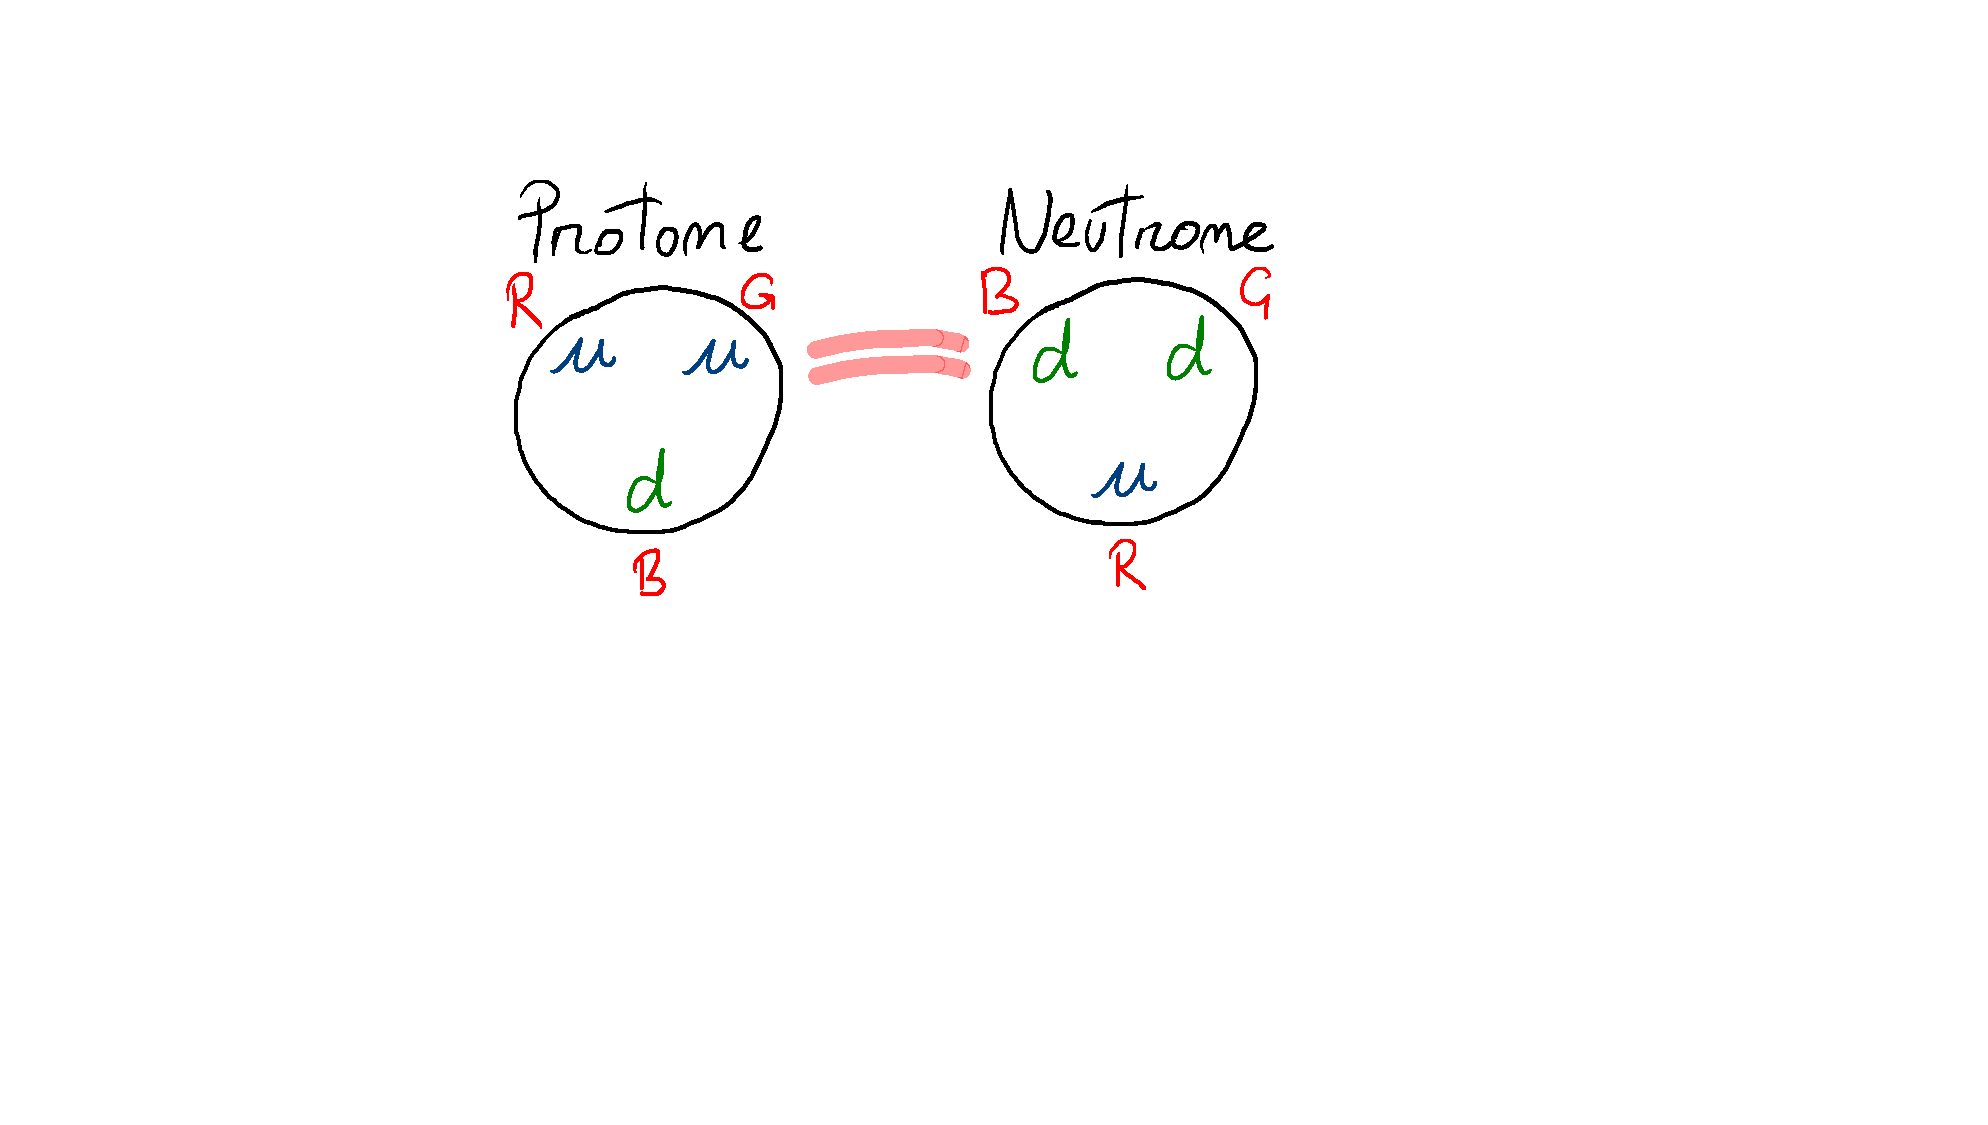
\includegraphics[scale=0.5]{/protone_neutrone_quark}
\caption{CAPTION}
\end{figure}

\paragraph{Carica di colore} I quark hanno anche un secondo tipo di carica: la \emph{carica di colore} che regola l'\emph{interazione forte} tra i quark.
La carica di colore può essere di tre tipi: Red (R), Green (G), Blue (B).
La somma delle tre cariche di colore dei rispettivi quark di un nucleone è nulla
\begin{equation}
R + G + B = 0
\end{equation}
un quark rosso (R) attira un quark verde (G) che attira un quark blu (B), mentre i quark dello stesso colore si respingono.
La teoria fondamentale della QCD esprime come l'interazione nucleare si possa interpretare come la carica di colore residua.

\paragraph{Il potenziale tra nucleoni} è un potenziale di interazione del tipo
%\begin{figure}[h]
%\centering
%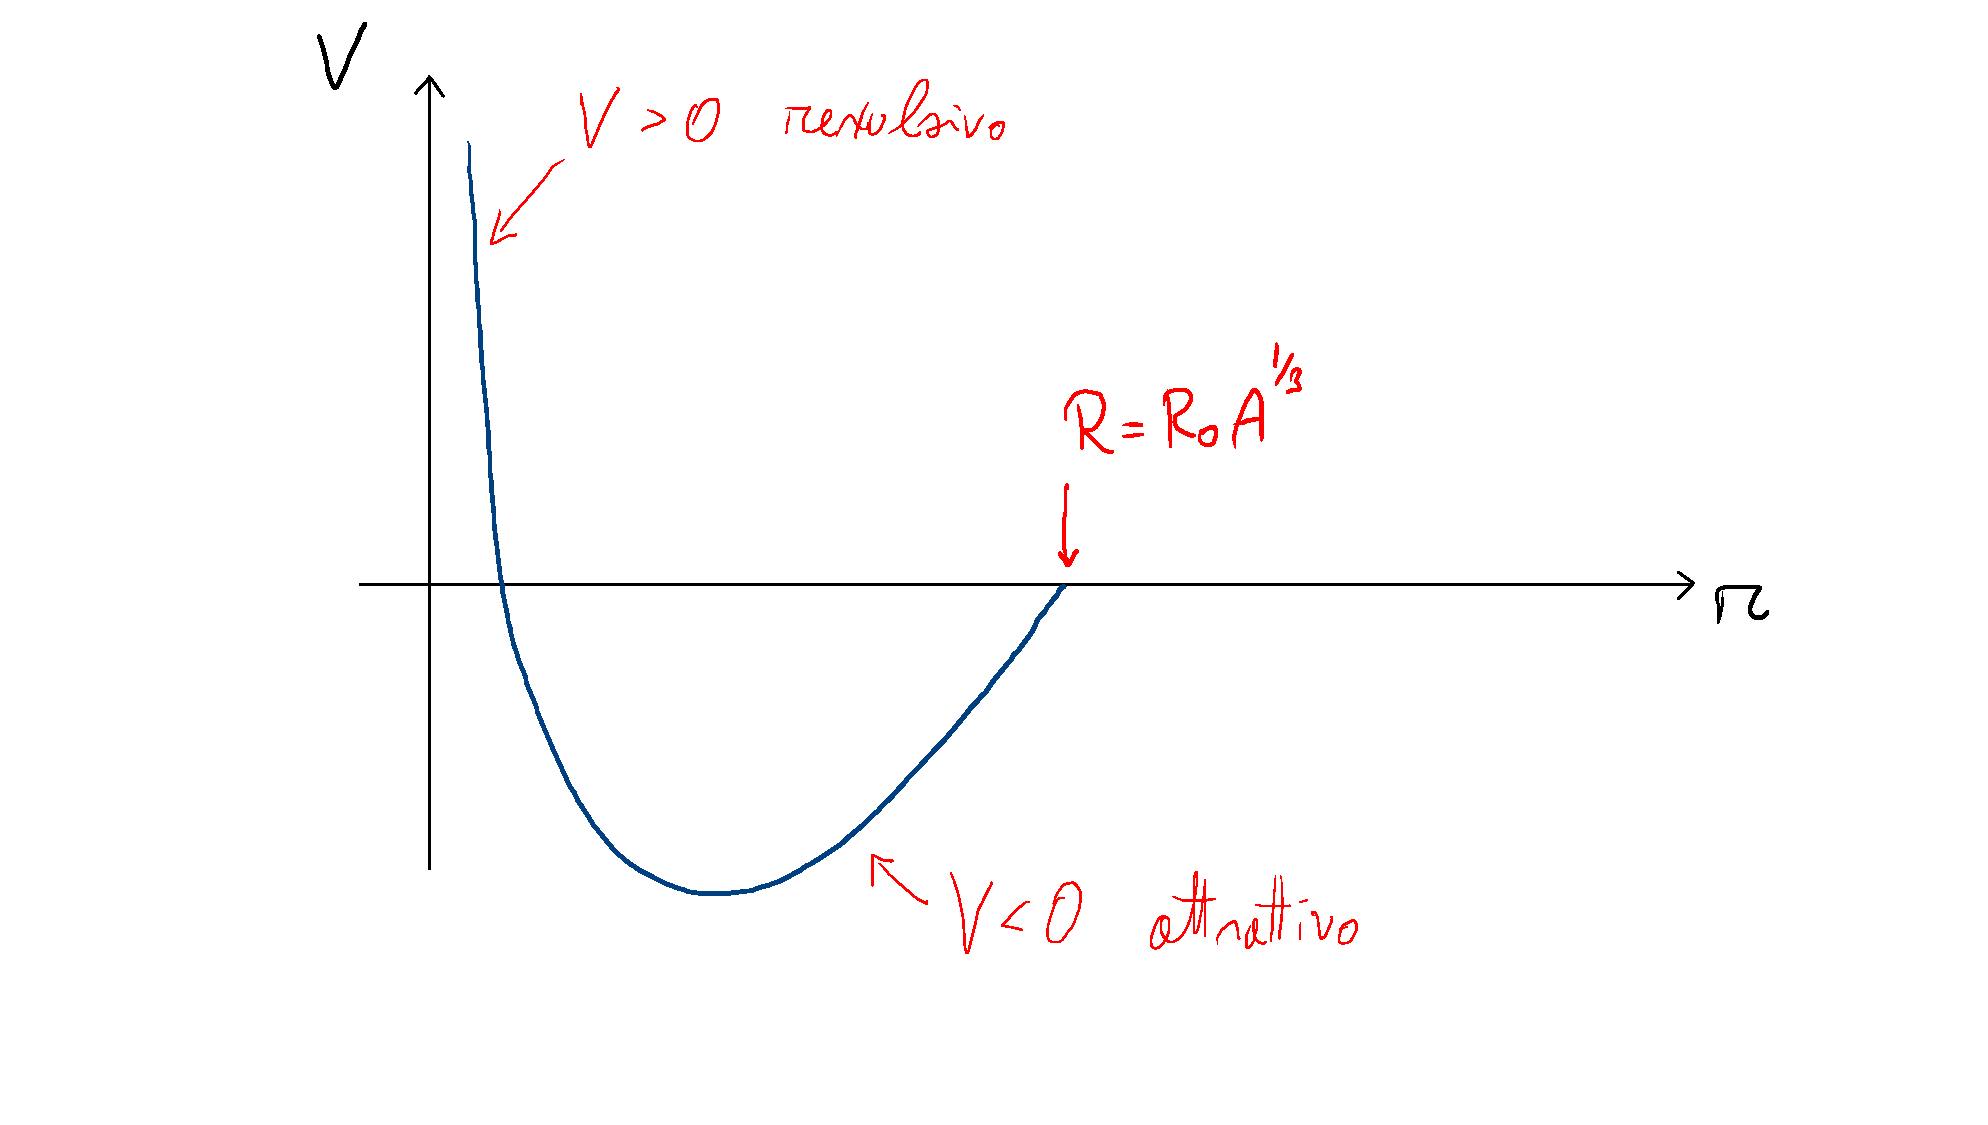
\includegraphics[scale=0.4]{/potenziale_nucleare_1}
%\caption{CAPTION}
%\end{figure}
Nella prima parte del potenziale si ha che per piccole distanze è \emph{positivo}, ovvero repulsivo, poiché altrimenti i nuclei \underline{privi di dimensione (?)} collasserebbero, ciò è legato al Principio di Esclusione di Pauli, nella seconda parte il potenziale è \emph{attrattivo} ed è ciò che "intrappola" i nucleoni all'interno del nucleo, inoltre oltre alla distanza data da $R = R_0 A^{\frac{1}{3}}$ la forza nucleare è nulla.

\paragraph{Il Deutone} è il nucleo del deuterio, è composto da un protone e un neutrone ed è il più semplice nucleo su cui studiare la forza nucleare.
Del deutone conosciamo l'energia di legame $E_B = \SI{-2.225}{MeV}$ e la distanza tra i nucleoni $R = \SI{2.1}{fm}$ ottenuti sperimentalmente.
Conosciamo inoltre che lo stato legato del deuterio è quello in cui gli spin sono paralleli, dato ottenuto dalla misurazione del momento magnetico, per cui lo spin del deutone è $S = 1$.
%\begin{figure}[h]
%\centering
%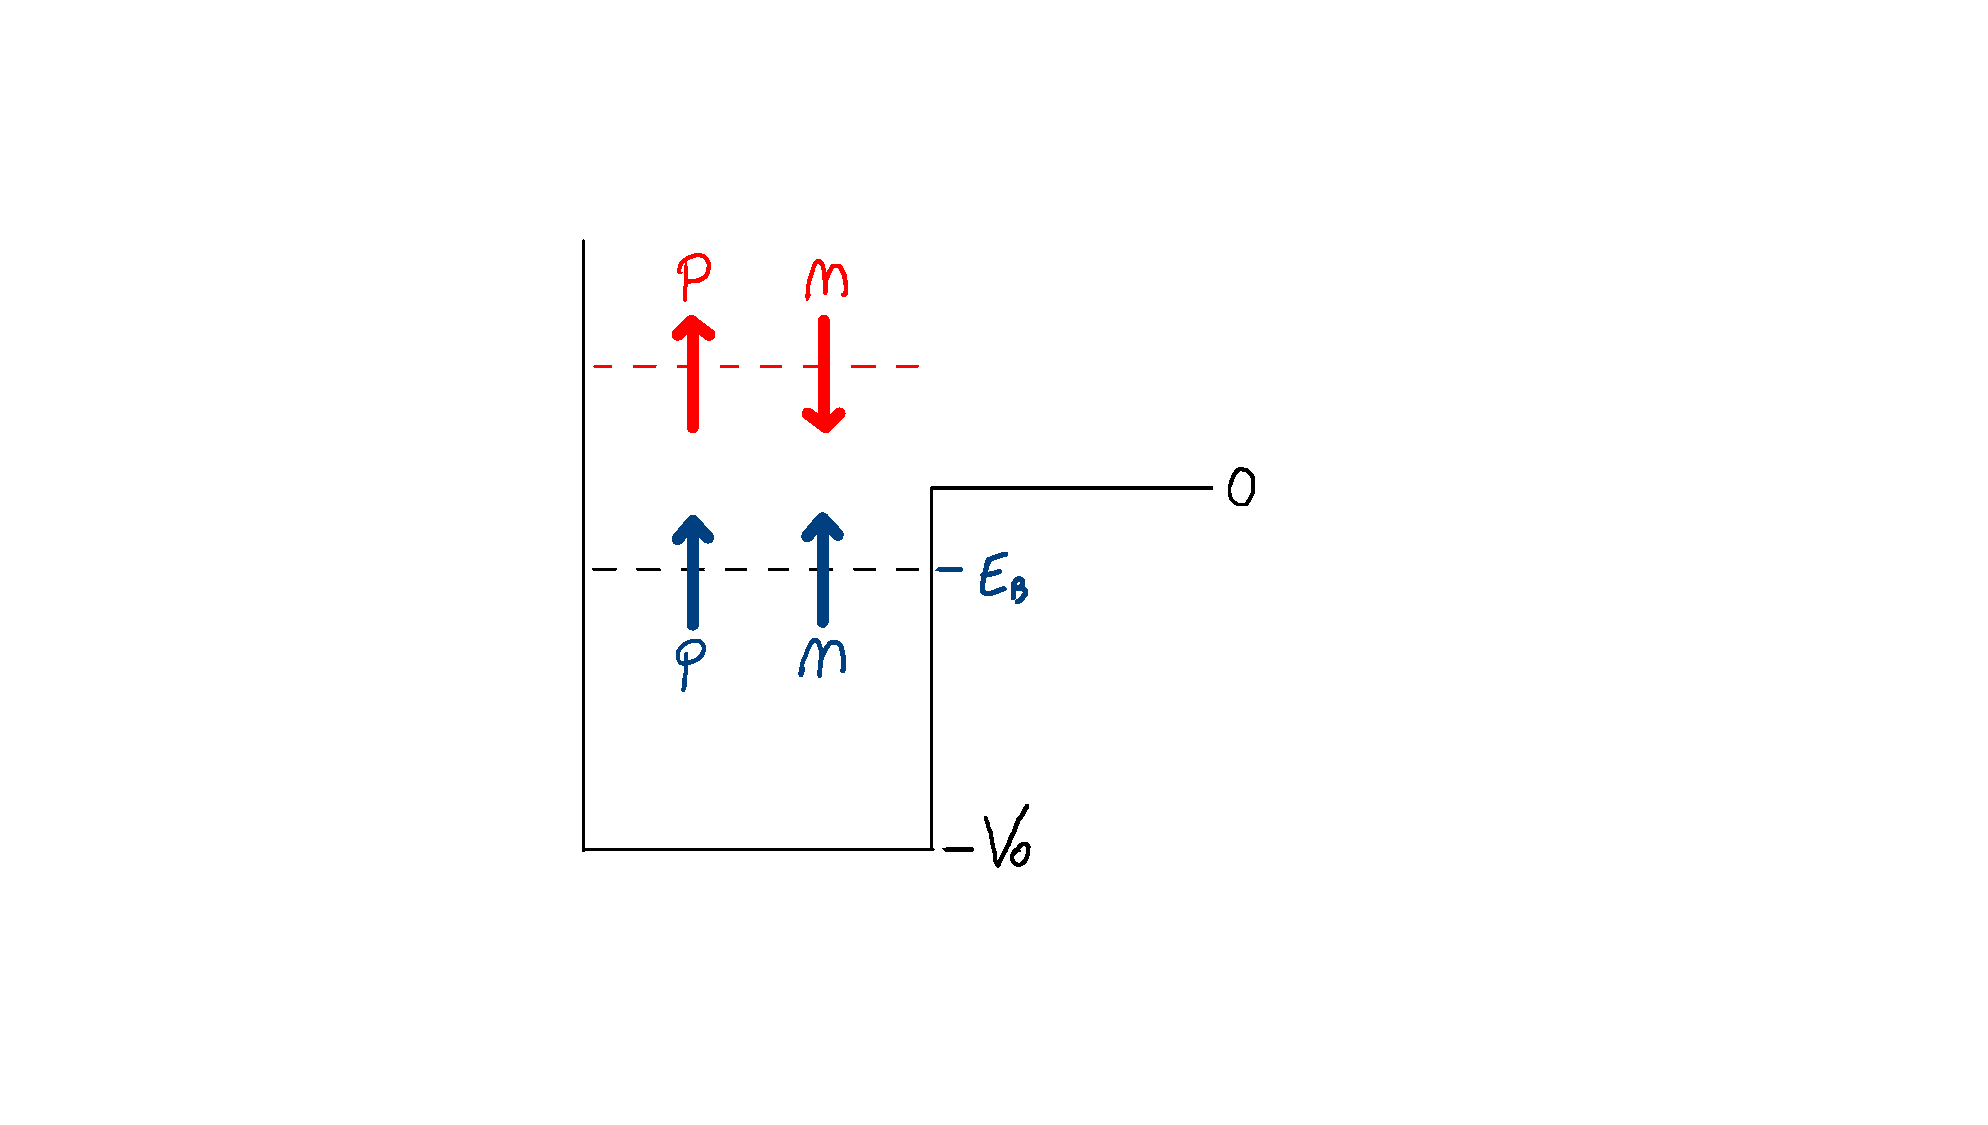
\includegraphics[scale=0.5]{/spin_deutone}
%\caption{CAPTION}
%\end{figure}
Uno stato con spin anti-parallelo corrisponde ad uno stato non legato, quindi fuori dalla buca di potenziale.
L'interazione nucleare dipende fortemente dallo spin.

Cerco ora il valore della buca di potenziale $V_0$, sommo l'energia cinetica $KE$ con l'energia potenziale $PE$
\begin{equation}
\begin{split}
E & = KE + PE \\
E_B & = KE + V_0
\end{split}
\end{equation}
scrivendo la funzione d'onda trovo il legame con il potenziale $V$
\begin{equation}
\begin{split}
H \psi & = E \psi \\
- \frac{\hbar^2}{2m} \frac{d^2}{dr^2} \psi + V \psi & = E \psi
\end{split}
\end{equation}
Il potenziale di questa buca è
\begin{equation}
V = 
\Bigg\{\begin{array}{l}
V_0 \quad\mbox{zona 1: dentro la buca} \\
0 \quad\mbox{ zona 2: altrove}
\end{array}
\end{equation}
Scrivo l'equazione di Schrodinger nella zona 1, in cui ho $V = V_0$
\begin{equation}
\begin{split}
- \frac{\hbar^2}{2m} \frac{d^2 \psi}{d r^2} + V_0 \psi & = E \psi \\
\frac{d^2 \psi}{d r^2} & = -\frac{2m}{\hbar^2} (E - V_0) \psi \\
\frac{d^2 \psi}{d r^2} & = - K^2 \psi \quad\quad \mbox{con } K^2 = \frac{2m}{\hbar^2} (E - V_0)
\end{split}
\end{equation}
la soluzione ha un andamento oscillatorio ed in generale è
\begin{equation}
\psi(r) = A \sin Kr + B \cos Kr
\end{equation}
calcolo $A$ e $B$ imponendo le condizioni al contorno:
\begin{equation}
\psi (0) = 0 \quad\Rightarrow\quad \psi(0) = A \sin 0 + B \cos 0 = 0 \quad\Rightarrow\quad B=0
\end{equation}
per cui diventa
\begin{equation}
\psi = A \sin K r
\label{psi_1}
\end{equation}
Scrivo l'equazione di Schrodinger nella zona 2, in cui ho $V =0$
\begin{equation}
\begin{split}
\frac{d^2 \psi}{d r^2} & = -\frac{2m}{\hbar^2} E \psi \\
\frac{d^2 \psi}{d r^2} & = L^2 \psi \quad\quad \mbox{con } L^2 = - \frac{2m}{\hbar^2} E
\end{split}
\end{equation}
la soluzione ha un andamento esponenziale ed in generale è
\begin{equation}
\psi(r) = C e^{L r} + D e^{- L r}
\end{equation}
di cui so che deve appartenere allo spazio di Hilbert, per cui la parte $e^{L r}$ non è soluzione in quanto non verifica la condizione $|\psi|^2 < \infty$, per cui diventa
\begin{equation}
\psi(r) = D e^{- L r} 
\label{psi_2}
\end{equation}
Eguagliando le funzioni d'onda \ref{psi_1} e \ref{psi_2} e le loro derivate in corrispondenza della frontiera $r = R$ trovo
\begin{equation}
\Bigg\{\begin{array}{l}
\psi_{1}(R) = \psi_{2}(R)\\
\psi_{1}'(R) = \psi_{2}'(R)
\end{array}
\quad\Rightarrow\quad 
\Bigg\{\begin{array}{l}
A \sin K R = D e^{ - L R }\\
K A \sin K R = -L D e^{ - L R }
\end{array}
\end{equation}
dividendo una con l'altra le equazioni del sistema trovo la relazione seguente in funzione dei parametri $K$ ed $L$
\begin{equation}
\begin{split}
K & = \sqrt{\frac{2m}{\hbar^2} (E - V_0)} \in \mathbb{R} \\
L & = \sqrt{- \frac{2m}{\hbar^2} E} \in \mathbb{R}
\end{split}
\end{equation}
che quindi diventa
\begin{equation}
\begin{split}
& K \cot K R = - L \\
& \sqrt{\frac{2m}{\hbar^2} (E - V_0)} \cot \Bigl[ R \sqrt{\frac{2m}{\hbar^2} (E - V_0)} \Bigr] = - \sqrt{- \frac{2m}{\hbar^2} E}
\end{split}
\end{equation}
da cui, inserendo i dati sperimentali, 
\begin{equation}
\begin{split}
E & = \SI{-2.225}{MeV} \\
R & = \SI{2.1}{fm}
\end{split}
\end{equation}
e la massa corrisponde alla massa ridotta tra il protone ed il neutrone
\begin{equation}
m = \frac{m_n m_p}{m_n + m_p} \simeq \frac{m_p^2}{2 m_p} = \frac{m_p}{2}
\end{equation}
trovo il valore della buca di potenziale
\begin{equation}
V_0 = \SI{-36}{MeV}
\end{equation}
(non è ben noto come sia davvero possibile risolvere l'equazione del tipo $x \cot a x = b$ ma ok, prendiamo atto del risultato precedente e andiamo avanti).

Risulta quindi che la buca di potenziale del Deutone è profonda $\SI{-36}{MeV}$ di cui solo $\SI{-2.225}{MeV}$ sono di energia potenziale, \emph{di legame}, mentre circa $\SI{-34}{MeV}$ sono di energia cinetica.

Per il ferro $^{56}_{26}Fe$ ad esempio si ha un'energia di legame media di circa $\SI{8}{MeV / nucleone}$, mentre
per il deutone $^{2}_{1}He$ si ha circa $\SI{1.1}{MeV / nucleone}$.

Troviamo tre punti notevoli della funzione d'onda:

\begin{itemize}
\item Quanto vale la funzione d'onda nel punto $r=R$?
In tale punto la funzione vale $\sin K R$ per cui conoscendo i dati trovo
\begin{equation}
\begin{split}
& R = \SI{2.1}{fm} \\
& K = \sqrt{ \frac{2m}{\hbar^2} (E - V_0) } \simeq \SI{0.9}{fm^{-1}} \\
& \sin K R = \sin (0.9 \cdot 2.1) = 0.95
\end{split}
\end{equation}

\item In che punto si ha il valore massimo della funzione d'onda?
\begin{equation}
\begin{split}
& \sin K r = 1 \\
& K r = \frac{\pi}{2} \\
& r = \frac{\pi}{2} \frac{1}{K} \simeq \SI{1.74}{fm}
\end{split}
\end{equation}

\item In che punto la funzione d'onda vale circa $\frac{1}{3}$?
\begin{equation}
\begin{split}
e^{ - L r } & \quad L = \sqrt{\frac{2mE}{\hbar^2}} \to \frac{1}{L} = \SI{4.4}{fm} \\
e^{ - L r } & \rightarrow e^{ \frac{-L}{L}} = e^{ -1 } = 0.37
\end{split}
\end{equation}
\end{itemize}
La funzione d'onda ottenuta evidenzia come sia possible trovare la particella al di fuori della buca di potenziale, a distanze oltre i $\SI{5}{fm}$.









